\documentclass[sigconf,review, anonymous]{acmart}
\acmConference[ICSE 2018]{40th International Conference on Software Engineering}{May 27--June 3, 2018}{Gothenburg, Sweden}
\acmYear{2018}

\usepackage{booktabs} % For formal tables
\usepackage{centernot}
\usepackage{algorithm}
\usepackage{algorithmic}
\usepackage{amsmath,amssymb,amsfonts}
\usepackage{balance}

\newtheorem{remark}{Remark}
\newtheorem{problem}{Problem}
\newtheorem*{running*}{Running example}
\usepackage[inline]{enumitem}
\settopmatter{printfolios=true}


\usepackage[xcolor=orange]{changes}
\definechangesauthor[name={Claudio Menghi},color=orange]{CM}
\definechangesauthor[name={Sergio Garcia},color=red]{SG}
%\definechangesauthor[name={Patrizio},color=blue]{PP}
\usepackage[colorinlistoftodos,prependcaption,textsize=tiny]{todonotes}
%\newcommand{\sergio}[1]{\todo[color=blue]{\textsf{SG} #1}}

\newboolean{showcomments}
\setboolean{showcomments}{true} % toggle to show or hide comments
\ifthenelse{\boolean{showcomments}}
{\newcommand{\nb}[2]{
  \fcolorbox{black}{yellow}{\bfseries\sffamily\scriptsize#1}
  {\sf\small$\blacktriangleright$\textit{#2}$\blacktriangleleft$}
 }
 \newcommand{\version}{\emph{\scriptsize$-$working$-$}}
}
{\newcommand{\nb}[2]{}
 \newcommand{\version}{}
}
\newcommand\patrizio[1]{\nb{Patrizio}{#1}}
\newcommand\claudio[1]{\nb{Claudio}{#1}}
\newcommand\sergio[1]{\nb{Sergio}{#1}}
\newcommand\jana[1]{\nb{Jana}{#1}}

\newcommand{\Sync}{\ensuremath{Meet}}
\newcommand{\cla}[1]{\textcolor{red}{{#1}}}
%%%shortcuts
\newcommand{\robotindex}{n}
\newcommand{\robotindexp}{m}
\newcommand{\setrobot}{\ensuremath{\mathcal{R}}}
\newcommand{\T}{\ensuremath{r}} %transition system

\newcommand{\powerset}{\raisebox{.15\baselineskip}{\Large\ensuremath{\wp}}}
\newcommand{\robot}{\ensuremath{\T}}

\newcommand{\INPUT}{\textbf{Input} }
\newcommand{\OUTPUT}{\textbf{Output} }

\newcommand{\AP}{\Pi} %atomic propositions
\newcommand{\service}{\pi}
\newcommand{\behavior}{\ensuremath{\mathcal{B}}} %Buchi automaton
\newcommand{\trace}{\ensuremath{\mathcal{T}}}
\newcommand{\A}{\ensuremath{\mathcal{A}}} %automaton
\newcommand{\B}{\ensuremath{\mathcal{B}}} %Buchi automaton
\newcommand{\BA}{B\"uchi automaton }
\renewcommand{\P}{\mathcal{P}} %product automaton
\newcommand{\R}{\mathcal{R}} %rabin automaton
\newcommand{\init}{\ensuremath{init}}
\newcommand{\pref}{\mathit{pref}}
\newcommand{\currs}{\mathfrak{s}}
\newcommand{\currq}{\mathfrak{q}}
\newcommand{\dur}{\Delta}
\newcommand{\wait}{\mathit{wait}}
\newcommand{\sync}{\mathit{sync}}
\newcommand{\nosync}{\mathit{nosync}}
\newcommand{\TS}{\ensuremath{\T=(S,} \ensuremath{\init}, \ensuremath{{A},} \ensuremath{\AP,} \ensuremath{T,} \ensuremath{\Sync,} \ensuremath{L)}}
\newcommand{\PTS}{\ensuremath{\T=(S,} \ensuremath{\init},   \ensuremath{{A},} \ensuremath{\AP,}    \ensuremath{T,}   \ensuremath{T_p,}  \ensuremath{\Sync}, \ensuremath{\Sync_p}, \ensuremath{L} )}
\newcommand{\PTSone}{\ensuremath{\T'=(S',} \ensuremath{\init',} \ensuremath{{A'},} \ensuremath{\AP',} \ensuremath{T',}  \ensuremath{T'_p,} \ensuremath{\Sync' )}}

\newcommand{\ra}{$\rightarrow$}
\newcommand{\ugh}[1]{\textcolor{red}{\uwave{#1}}} % please rephrase
\newcommand{\ins}[1]{\textcolor{blue}{\uline{#1}}} % please insert
\newcommand{\del}[1]{\textcolor{red}{\sout{#1}}} % please delete
\newcommand{\chg}[2]{\textcolor{red}{\sout{#1}}{\ra}\textcolor{blue}{\uline{#2}}}

\newcommand{\TSprime}{{\T'=(S',\init',{A}',T', \Sync')}}

\newcommand{\TSoneprime}{{\T_1=(S'_1, \init'_{1},{A}'_1,T'_1, \Sync')}}

\newcommand{\TSone}{{\T_1=(S_1,\init_{1},{A}_1,T_1, \Sync_1)}}
\newcommand{\TStwo}{{\T_1=(S_2, \init_{2},{A}_2,T_2, \Sync_2)}}
\newcommand{\TSproduct}{{(S_1 \times S_2,\langle \init_{1}, s_{2,\init} \rangle,{A}_2 \cup {A}_2,T, \Sync)}}
\newcommand{\TStwoprime}{{\T_1=(S'_2,\init'_{2},{A}'_2,T'_2)}}
\newcommand{\robotpar}{\ensuremath{\T_\robotindex=} \ensuremath{(S_\robotindex,} \ensuremath{\init_{\robotindex},} \ensuremath{{A}_\robotindex,} \ensuremath{\AP_\robotindex ,} \ensuremath{T_\robotindex,} \ensuremath{\Sync_\robotindex)}}
\newcommand{\robotp}[1]{\ensuremath{\T_{#1}=} \ensuremath{(S_{#1},} \ensuremath{\init_{#1},} \ensuremath{{A}_{#1},} \ensuremath{\AP_{#1} ,} \ensuremath{T_{#1},} \ensuremath{\Sync_{#1})}}
\newcommand{\partialrobotp}[1]{\ensuremath{\T_{#1}}=(\ensuremath{S_{#1}}, \ensuremath{\init_{#1},} \ensuremath{{A}_{#1},} \ensuremath{\AP_{#1},} \ensuremath{T_{#1},} \ensuremath{T_{p,#1},} \ensuremath{\Sync_{#1},} 
\ensuremath{\Sync_{p,#1}}, \ensuremath{{L}_{#1}})}


\newcommand{\PTSpar}{\ensuremath{\T_\robotindex=(S_\robotindex,} \ensuremath{\init_{\robotindex},} \ensuremath{{A}_\robotindex,} \ensuremath{\AP_\robotindex ,} \ensuremath{T_\robotindex,} \ensuremath{T_{p,\robotindex},} \ensuremath{\Sync_\robotindex}, 
\ensuremath{\Sync_{p,\robotindex}, \ensuremath{L}_\robotindex)}}

\newcommand{\network}{\ensuremath{\N}}
\newcommand{\robotapplication}{\ensuremath{\N}}
\newcommand{\robotset}{\network = \{\ensuremath{\robot_1,} \ensuremath{\robot_2, \ldots}, \ensuremath{\robot_N\}}}
\newcommand{\robotsetdef}{\{\ensuremath{\robot_1,} \ensuremath{\robot_2, \ldots}, \ensuremath{\robot_N\}}}
\newcommand{\robotsetdefp}{\{\ensuremath{\robot'_1,} \ensuremath{\robot'_2, \ldots}, \ensuremath{\robot'_N\}}}
\newcommand{\property}{\ensuremath{\phi}}
\newcommand{\missions}{\ensuremath{\Phi}}
\newcommand{\propertiesset}{\ensuremath{\Phi =} \{\ensuremath{\property_1,} \ensuremath{\property_2, \ldots}, \ensuremath{\property_N\}}}


\newcommand{\TSi}{{\T_i=(S_i,\init_{i},{A_i} ,T_i)}}
\newcommand{\N}{\mathcal{H}}
\newcommand{\M}{{M}}
\newcommand{\model}{\mathcal{M}}
\newcommand{\I}{\mathcal{I}}
\newcommand{\D}{{D}}
\renewcommand{\O}{\mathcal{O}}

\newcommand{\toolName}{MAPmAKER}
\newcommand{\APs}{\mathbf{\Pi}}
\newcommand{\Lang}{\mathcal{L}} %language
\newcommand{\Set}{\mathsf{S}} %set
\newcommand{\Spec}{\mathbf{\Phi}}
\newcommand{\Epsilon}{\mathcal{E}}
\renewcommand{\i}{\iota}
\newcommand{\Nat}{\mathbb{N}} %natural numbers
\newcommand{\Real}{\mathbb{R}}
\newcommand{\Next}{\mathsf{X}}
\newcommand{\Until}{\mathsf{U}}
\newcommand{\Always}{\mathsf{G}}
\newcommand{\Event}{\mathsf{F}}
\newcommand{\false}{\mathit{false}}
\newcommand{\true}{\mathit{true}}
\newcommand{\trueval}{\ensuremath{\top}}
\newcommand{\falseval}{\ensuremath{\bot}}
\newcommand{\maybe}{\ensuremath{?}}
\renewcommand{\epsilon}{\varepsilon}
\newcommand{\prop}{\pi}
\newcommand{\ie}{{i.e., }}
\newcommand{\eg}{{e.g., }}
\newcommand{\progressive}{\varpi}
\newcommand{\move}{\mathit{move}}
\newcommand{\h}{h}
\renewcommand{\H}{H}
\newcommand{\parti}{\mathit{P}}
\newcommand{\Alpha}{\mathbf{\Sigma}}
\renewcommand{\mod}{\mathrm{\, mod \, }}
\newcommand{\suc}{\mathit{succ}}
\newcommand{\dist}{\mathrm{dist}}
\newcommand{\proj}{\mathrm{proj}}
\newcommand{\parspace}{\vskip 0.05in}


\makeatletter
\newcommand*{\da@rightarrow}{\mathchar"0\hexnumber@\symAMSa 4B }
\newcommand*{\da@leftarrow}{\mathchar"0\hexnumber@\symAMSa 4C }
\newcommand*{\xdashrightarrow}[2][]{%
  \mathrel{%
    \mathpalette{\da@xarrow{#1}{#2}{}\da@rightarrow{\,}{}}{}%
  }%
}
\newcommand{\xdashleftarrow}[2][]{%
  \mathrel{%
    \mathpalette{\da@xarrow{#1}{#2}\da@leftarrow{}{}{\,}}{}%
  }%
}
\newcommand*{\da@xarrow}[7]{%
  % #1: below
  % #2: above
  % #3: arrow left
  % #4: arrow right
  % #5: space left 
  % #6: space right
  % #7: math style 
  \sbox0{$\ifx#7\scriptstyle\scriptscriptstyle\else\scriptstyle\fi#5#1#6\m@th$}%
  \sbox2{$\ifx#7\scriptstyle\scriptscriptstyle\else\scriptstyle\fi#5#2#6\m@th$}%
  \sbox4{$#7\dabar@\m@th$}%
  \dimen@=\wd0 %
  \ifdim\wd2 >\dimen@
    \dimen@=\wd2 %   
  \fi
  \count@=2 %
  \def\da@bars{\dabar@\dabar@}%
  \@whiledim\count@\wd4<\dimen@\do{%
    \advance\count@\@ne
    \expandafter\def\expandafter\da@bars\expandafter{%
    }%
  }%  
  \mathrel{#3}%
  \mathrel{%   
    \mathop{\da@bars}\limits
    \ifx\\#1\\%
    \else
      _{\copy0}%
    \fi
    \ifx\\#2\\%
    \else
      ^{\copy2}%
    \fi
  }%   
  \mathrel{#4}%
}

\everymath{\vadjust{\nobreak\null}}

\makeatletter
\def\old@comma{,}
\catcode`\,=13
\def,{%
  \ifmmode%
    \old@comma\discretionary{}{}{}%
  \else%
    \old@comma%
  \fi%
}
\makeatother

\def\HiLi{\leavevmode\rlap{\hbox to \hsize{\color{yellow!50}\leaders\hrule height .8\baselineskip depth .5ex\hfill}}}

\newif\ifextended
\extendedfalse
%\extendedtrue

\ifextended
\newcommand{\extended}[1]{\textcolor{red}{#1}} 
\newcommand{\notextended}[1]{}
\else
\newcommand{\extended}[1]{}
\newcommand{\notextended}[1]{#1}
\fi

\begin{document}
\title{Multi-Robot LTL Planning Under Uncertainty}


%\author{Claudio Menghi}
%\affiliation{%
%  \institution{Institute for Clarity in Documentation}
%  \streetaddress{P.O. Box 1212}
%  \city{Dublin} 
%  \state{Ohio} 
%  \postcode{43017-6221}
%}
%\email{trovato@corporation.com}
%
%\author{Patrizio Pelliccione}
%\affiliation{%
%  \institution{Institute for Clarity in Documentation}
%  \streetaddress{P.O. Box 1212}
%  \city{Dublin} 
%  \state{Ohio} 
%  \postcode{43017-6221}
%}
%\email{webmaster@marysville-ohio.com}



\begin{abstract}
Robot applications are increasingly based on \emph{teams} of autonomous robots that collaborate and interact to perform a desired mission. 
Such applications ask for decentralized techniques that allow for tractable automated planning. %that are \emph{decentralized}, i.e., they decompose the team of robots into classes that have missions that can be analyzed in isolation inside each class.
Another aspect that %novel 
state-of-the-art robot applications must consider is \emph{partial knowledge} about the environment in which the robots are operating and the associated uncertainty with the outcome of the robots' actions.
This occurs, for example, when robots navigate in environments affected by natural disasters, where the movement between locations %or the execution of specific actions 
may be impossible due to structural collapses, flooding, etc.

Current planning techniques used for teams of robots that should perform complex missions do not systematically address these challenges: they are either based on centralized solutions and hence not scalable, they consider rather simple missions, such as A-to-B travel, or do not work in partially known environments. 
We present a %novel 
planning solution that decomposes the team of robots into subclasses, considers complex high-level missions given in temporal logic, %is \emph{decentralized} 
and at the same time works when only \emph{partial knowledge} of the environment is available.
We prove the correctness of the solution and evaluate its effectiveness on a set of realistic examples.
\end{abstract}

%
% The code below should be generated by the tool at
% http://dl.acm.org/ccs.cfm
% Please copy and paste the code instead of the example below. 
%
%\begin{CCSXML}
%<ccs2012>
% <concept>
%  <concept_id>10010520.10010553.10010562</concept_id>
%  <concept_desc>Computer systems organization~Embedded systems</concept_desc>
%  <concept_significance>500</concept_significance>
% </concept>
% <concept>
%  <concept_id>10010520.10010575.10010755</concept_id>
%  <concept_desc>Computer systems organization~Redundancy</concept_desc>
%  <concept_significance>300</concept_significance>
% </concept>
% <concept>
%  <concept_id>10010520.10010553.10010554</concept_id>
%  <concept_desc>Computer systems organization~Robotics</concept_desc>
%  <concept_significance>100</concept_significance>
% </concept>
% <concept>
%  <concept_id>10003033.10003083.10003095</concept_id>
%  <concept_desc>Networks~Network reliability</concept_desc>
%  <concept_significance>100</concept_significance>
% </concept>
%</ccs2012>  
%\end{CCSXML}
%
%\ccsdesc[500]{Computer systems organization~Embedded systems}
%\ccsdesc[300]{Computer systems organization~Redundancy}
%\ccsdesc{Computer systems organization~Robotics}
%\ccsdesc[100]{Networks~Network reliability}


%\keywords{ACM proceedings, \LaTeX, text tagging}


\maketitle

\section{Introduction}
Robotic applications usually rely on a set of robots that are used to perform missions.
The term mission can refer to a \emph{global mission}, i.e., the high-level mission that must be accomplished by the whole team~\cite{quottrup2004multi} or a \emph{local mission}, i.e., the mission that should be achieved by a single robot, possibly by collaborating with other robots~\cite{tumova2016multi}.
%Every robot is commanded to achieve a local mission, specified as a LTL property.
Planners are one of the main ingredients that allow robots to achieve  missions.
A \emph{planner} is  a software component that receives as input a model of the robotic application and computes  a set of actions---a \emph{plan}---that, if performed, allows the achievement of a desired mission~\cite{latombe2012robot}.
Recent works in robotics have defined robot applications using finite transition systems and some of them define their local missions as a Linear-time Temporal Logic (LTL) property (e.g., \cite{menghi2018multi,guo2015multi,tumova2016multi}).
%\del{LTL enables the enrichment of the specification of temporal goals that are used as input for planners.}

Current robotic applications require planners to address two main challenges: 
\begin{enumerate*}
%\claudio{I am just a bit concern about the term Tractability since Mapmaker does not make the problem tractable. I suggest to remove it and just focus on decentralization.}
\item the planning algorithm should work when (only) partial knowledge about the system---including the robots and their working environment---is present;
\item the planning problem should be solved by decentralized algorithms that helps to reduce the planning overhead.
\end{enumerate*}


%\sergio{in the following paragraphs I cite several works to speak trying to give some background but also related work. Is it enough?}

%Tractability refers to the capability of computer algorithms in solving problems. \claudio{I suggest to delete the previous sentence}
Several works studied centralized planners that are able to manage \emph{teams} of robots that collaborate to achieve a certain goal (a global mission)~\cite{kloetzer2011multi,quottrup2004multi}.
However, this methodology planning is computationally expensive, especially when the number of robots within the team increases % \patrizio{do we have a measure for the size when the problem is becoming difficult with existing planners?} 
and they need to collaborate to fulfill their local missions.
For this reason, research interest had focused on decomposing a global mission into a set of local missions to be achieved by each robot of the team~\cite{schillinger2016decomposition,guo2015multi,tumova2016multi}. 
These local missions have been recently exploited by \emph{decentralized} planners~\cite{tumova2016multi}, i.e., planners that instead of evaluating the global mission over the whole team of robots, analyze the satisfaction of local missions inside a subset of the team of robots. 
In this way, the problem of finding a collective team behavior is decomposed into sub-problems that avoid the expensive fully centralized planning. 
However, the applicability of these algorithms has never been studied when only partial knowledge about the system is available.



The role of partial knowledge in software development has been strongly studied in literature.
Research has been done on how to consider partial knowledge in requirement analysis and elicitation~\cite{menghi2017integrating,menghi2017cover,letier2008deriving}, in the development of a model of the system that satisfies a set of desired properties~\cite{uchitel2009synthesis,uchitel2013supporting,famelis2012partial,albarghouthi2012under,Bernasconi2017}, and in checking   whether an  already designed model possesses some properties of interest~\cite{menghi2016dealing,bruns1999model,chechik2004multi}.
However, most of the existing planners assume that the environment in which the robots are deployed is known~\cite{7139412}. 
This assumption does not usually hold in real-word scenarios~\cite{lahijanian2016iterative},  where, for example,  the robots navigate in environments affected by natural disasters, where the movement between locations or the execution of specific actions may be impossible. %due to structural collapses, flooding, etc.
The planners that consider  partial information about the environment in which the robots operate (e.g.,~\cite{roy2006planning,du2012robot,diaz2001exploring}) usually rely on probabilistic algorithms and are not  \emph{decentralized}.
%However, %to the best of our knowledge, 
%literature considering \emph{decentralized} planners %have not been applied when 
%with only partial knowledge about the robot application and temporal logic goals
%is rather limited \cite{guo2015multi}.

%Nowadays, most of the planners consider the model of the environment as known and not dynamic~\cite{7139412}. 
%However, this is not a real condition of real world scenarios
%In real scenarios the knowledge of the environment cannot be ensured, so only \emph{partial knowledge} is available.
%For this reason, there is an increasing need of tools able to compute a plan even when only partial information of the environment is available, as seen in \cite{roy2006planning,du2012robot,diaz2001exploring}.


%As seen in \cite{tumova2016multi}, this collaborative fashion of accomplishing the global mission is performed in a \emph{decentralized} way.
%Each robot that is part of a subset of the team computes the solution for its own sub-mission, avoiding the expensive %fully centralized planning and making it more robust to local problems.
%\toolName\ splits the given set of robot that conforms the team into classes depending on the local mission that each of them must achieve.

This work presents  \toolName: a Multi-robot plAnner for PArtially Known EnviRonments.
 \toolName\ provides a  \emph{decentralized} planning solution that works in \emph{partially known} environments.
%\toolName\ modifies~\cite{tumova2016multi} by supporting partial knowledge.
Decentralization is realized by decomposing the robotic team into subteams based on their missions, and then by running a classical planning algorithm.
Partial knowledge is handled by calling twice a classical planning algorithm.
The theory that supports \toolName\ including proofs of correctness, a detailed description of the modelling formalisms and the verification procedures can be found in~\cite{menghi2018multi}.
In this paper we present the implementation of \toolName\ , the component that compounds it, the models it uses, how it can be used,  and  show how planners can deal with the previously stated features. 
We also provide a demonstration video to illustrate such concepts.
In this sense the contribution is more a proof of concept than a tool ready to be used for real-world scenarios.
\toolName~builds upon the planner proposed by Tumova et al.~\cite{tumova2016multi}.
It is evaluated by analysing its behaviour on a robot application simulating a hospital environment with the presence of uncertainty.
%obtained from the RobotCup Logistics League competition~\cite{karrasrobocup} and on a robotic application working in an apartment of about 80 m$^2$~\cite{map}.
%, which is part ofa large residential facility for senior citizens.
\toolName\  together with 
\begin{enumerate*}
\item a complete replication package,
\item a set of videos showing \toolName\ in action computing and solving the scenario presented at the previous bullet, and
\item a brief user guide that defines the main functionalities 
\end{enumerate*}
 are available at our Github repository~\cite{repo}. %~\url{https://github.com/claudiomenghi/MAPmAKER/}. 


%This paper is organized as follows. 
%Section~\ref{sec:approach} presents an overview of \toolName.
%Section~\ref{sec:tool} describes how  \toolName\ can be used.
%Section~\ref{sec:evaluation} evaluates  \toolName.
%Section~\ref{sec:conclusion} concludes with final remarks.



\section{Running Example}
\label{sec:running}
A set $R=\{r_1, r_2, r_3 \}$ of robots  is deployed in the environment graphically described in  Fig.~\ref{fig:example1}.
This environment represents a building made by four rooms $L=\{ l_1, l_2, l_3, l_4 \}$, which has been affected by an earthquake.
The environment is further partitioned in cells, each labeled with an identifier in $c_1, c_2, \ldots, c_{30}$.
Robots $r_1$, $r_2$, and $r_3$ are placed in their initial locations.
Each robot is able to move from one cell to another, by performing action $mov$.
The robots are also able to perform the following actions.
Robot $r_1$ is able to load debris of the building by performing action $ld$. 
In Fig.~\ref{fig:example1} the cells in which a robot $r$ can perform an action $\alpha$ are marked with the label $r(\alpha)$.
Robot $r_2$ can wait until another robot loads debris on it by performing action $rd$ and can unload debris by performing one of the two actions $ud1$ and $ud2$. 
Actions $ud1$ and $ud2$ use different actuators.
Specifically, action $ud1$ uses a gripper while action $ud2$ exploits a dump mechanism.
Robot $r_3$ is able to take pictures by performing action $tp$ and send them using a communication network through the execution of action $sp$. 
Symbols $r_1(ld)$, $r_2(rd)$, $r_2(ud1)$, $r_2(ud2)$, $r_3(tp)$, and $r_3(sp)$ are used in Fig.~\ref{fig:example1} to mark the regions where  actions can be executed by the robots, while movement actions are not reported for graphical reasons.
Each action may be associated with a service, which is a high-level functionality provided by the robot when an action is performed.
For example, actions $ld$, $rd$, $tp$, and $sp$  are associated with the services \emph{load\_carrier}, \emph{detect\_load}, \emph{take\_snapshot}, and \emph{send\_info}, respectively.
Actions $ud1$ and $ud2$ are associated with service \emph{unload}.
The labels $L(\pi,\alpha)=\trueval$ below Fig.~\ref{fig:example1} are used to indicate that a service $\pi$ is associated with  action $\alpha$. 
Robots must meet and  synchronously execute actions. 
In this example, robots $r_1$ and  $r_2$ must meet  in cell $c_7$ and synchronously execute actions $ld$ and $rd$, respectively. 
The cells where meeting is requested are marked with rotating arrows marked with the identifiers of the robots that must meet, meaning that, in order to meet, the robots must be on the same cell to meet.


\begin{figure}[!t]
\begin{center}
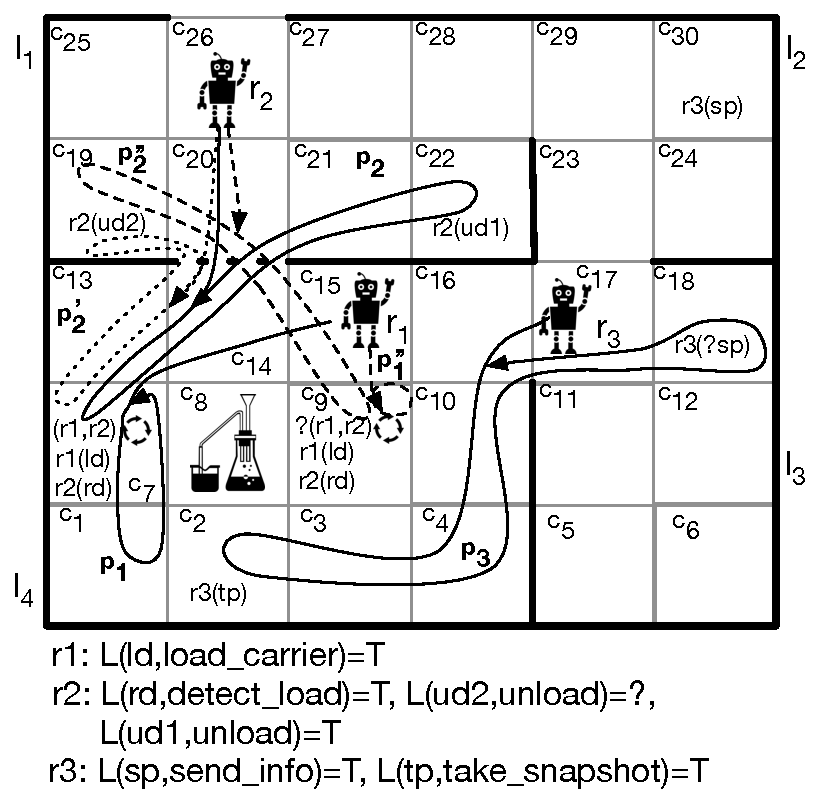
\includegraphics[width=0.9\linewidth]{Figures/motivatingExample.pdf}
\caption{An example showing the model of the robots and their environment. Plans computed by \toolName\ are represented by trajectories marked with arrows.}
\label{fig:example1}
\end{center}
\end{figure}

The \emph{mission}  the team of robots has to achieve is to check whether toxic chemicals have been released by the container located in $l_4$.
We assume that the mission is specified through a set of \emph{local missions} assigned to each robot of the team and described in Linear Time Temporal Logic  (LTL).
An LTL formula is obtained by composing actions with standard LTL operators: $\Next$ (next), $\Event$  (eventually),  $\Always$ (always) and $\Until$ (until)~\cite{pnueli1977temporal}. 
In our example the mission  can be specified by means of the following local missions: $\phi_1=\Always (\Event ($\emph{load\_carrier}$))$, 
$\phi_2=\Always (\Event($\emph{detect\_ load} $ \wedge \Event ($\emph{unload}$)))$, 
 $\phi_3=\Always ( \Event ($\emph{take\_snapshot} $\wedge \Event ($\emph{send\_info}$)))$, which are assigned to robot $r_1$, $r_2$ and $r_3$, respectively.
The formulae specify that periodically robot $r_1$ loads debris on $r_2$ (by performing action \emph{load\_carrier}), robot $r_2$ receives debris (when action \emph{detect\_ load} occurs)  and brings them to an appropriate unload area (by performing action \emph{unload}), and robot $r_3$ continuously takes pictures (by performing action \emph{take\_snapshot}) and sends them using the communication network (by performing action \emph{send\_info}).
Informally, while $r_3$ continuously takes pictures and sends them using the communication network, $r_1$ and $r_2$ remove debris to allow $r_3$ having a better view on the container.
The pictures allow verifying whether toxic chemicals have been released by the container.

The presence of partial knowledge about the robots and their environment is described in the following.

\textbf{Partial knowledge about the actions execution.} 
The robots can move between cells separated by grey lines, while they cannot cross black bold lines.
It is unknown whether it is possible to move between cells $c_{14}$ and $c_{20}$ since the structure may have been affected by collapses.
This is indicated using a dashed black bold line.
It is also unknown whether robot $r_3$ can send pictures using a communication network in location $l_3$ and specifically in cell $c_{18}$, i.e., whether action $s_p$ can be performed. 
Locations of the environment where it is unknown if an action can be provided are marked with the name of the action preceded by symbol $?$.

\textbf{Unknown service provisioning.} 
There are cases in which actions can be executed but there is uncertainty about service provisions.
For example, actions $ud1$ and $ud2$ of robot $r_2$ unload the robot.
Action $ud2$ will always be able to provide the \emph{unload} service, while it is unknown whether $ud1$ is actually able to provide this service since its effectiveness depends on the size of the collected debris. 
 In Fig.~\ref{fig:example1}, the label $L(ud1,unload)=?$ indicates that there is partial knowledge  about the provision of the \emph{unload} service when action $ud1$ is performed. 

\textbf{Unknown meeting capabilities.} 
It is  unknown whether robots $r_1$ and $r_2$ can meet in one cell of the environment. 
For example, a collapse in the roof of the building may forbid the two robots to concurrently execute services $ld$ and $rd$, i.e., there is not enough space for $r1$ to load $r2$. 
Unknown meeting capabilities are indicated with rotating arrows labeled with the symbol $?$.
For example,  in Fig.~\ref{fig:example1}, it is unknown whether robots $r_1$ and $r_2$ are able to meet in cell $c_{9}$.




\section{Related work}
\label{sec:related}
\emph{Decentralized solutions.}
Decentralized planning problem has been studied for known environments~\cite{schillinger2016decomposition,guo2015multi,tumova2016multi}.
However, planners for partially known environments do not usually employ decentralized solutions~\cite{roy2006planning,du2012robot,diaz2001exploring}. 

\emph{Dealing with partial knowledge in planning.}
Planning in partially known environments is handled in different ways. 
\begin{enumerate*}
\item Several works (e.g.,~\cite{ding2011ltl,kurniawati2011motion,wolff2012robust,du2012robot,Roy2006,chen2012ltl,nikou2017probabilistic,7078886,7139350,narayanan2015task}) consider probabilities within the planning algorithm.
Most of these works  treat partial information by modeling the robotic application using some form of \emph{Markov decision processes} (MDP).
In some of these works~\cite{ding2011ltl,chen2012ltl} transitions of the robots are associated with probabilities which indicate the probability of reaching the destination of the transition given that an action is performed.
In other works~\cite{wolff2012robust}, transition probabilities are not exactly known but are known to belong to a given uncertainty sets.
Finally, several works~\cite{kurniawati2011motion,Roy2006} consider partially observable Markov decision processes.
All these approaches generally generate plans that maximize the worst-case probability of satisfying a mission.
Differently, our work does not consider probabilities.
\item Several works (e.g,~\cite{lahijanian2016iterative,livingston2012backtracking,l2014safety,nie2016searching,7139412}) studied how to change the planned trajectories when unknown obstacles are detected or when obstacles move in a unpredictable way.
In this case, the used underlying model is some sort of \emph{hybrid model}, i.e., models in which finite state machines are combined with differential equations. 
In~\cite{lahijanian2016iterative}, to plan trajectories the authors use a high-level planner that exploits an abstraction of the hybrid system and the mission to compute high-level plans. 
The low-level planner uses the dynamics of the hybrid system and the suggested high-level plans to explore the state space for feasible solutions.
Every time an unknown obstacle is encountered, the high-level planner modifies the coarse high-level plan online by accounting for the geometry of the discovered obstacle. 
Within this framework, \toolName\ can be considered as a high-level planner that is able to use an abstraction of the hybrid system that contains partial information, i.e., encode unknown obstacles.
\item Some  approaches  analyzed how to update plans when new information about known model of a robotic application is detected (e.g.,~\cite{guo2015multi}). 
Differently, in our approach portions of the model of the robotic application are partially known,  partial knowledge is reduced as true and false evidence about partial information is detected.
Other works (e.g.,~\cite{7139310}), aim at detecting how to explore totally unknown environments.
\item 
Plan synthesis is a particular instance of controller synthesis. 
Controller  synthesis (e.g.,~\cite{cassandras2009introduction,D'ippolito:2013:SNE:2430536.2430543}) aims at finding a component, usually indicated as controller or supervisor, that ensures property satisfaction for all the possible system executions.
Differently, plan synthesis aims at finding a single execution, i.e., a plan that ensures property satisfaction.
The controller synthesis  is usually (\cite{kress2009temporal,wongpiromsarn2009receding,chen2012ltl,livingston2012backtracking,guo2013revising}) performed by solving a two player game between robots and their environment.
The goal is to find a strategy the robots can use that allows always winning the game.
Differently, in our case the planning algorithm ensures that there is a way of completing the \emph{single} (possible) plan that satisfies the property of interest. 
\item \toolName\ can be classified on the boundary between reactive synthesis~\cite{chen2012ltl,livingston2012backtracking,thomas2002automata} techniques and iterative planning~\cite{guo2013revising,maly2013iterative}. 
As reactive synthesis techniques, \toolName\ constructs a control strategy that accounts for every possible variation in the environment, but the computed plan does not allow always winning the  \emph{two player game} between the robots and their environment.
As  iterative planning, a new plan is computed on-the-fly when new information is available.
\end{enumerate*}
%\sergio{probably you did it on purpose for reaching the 10 pages, but the last paragraph is huge and it makes harder following the text }


\section{Conclusions}
\label{sec:conclusion}
We presented  \toolName, a  decentralized planner for partially known environments.
%\del{The theoretical results show that any planner can be used within \toolName. %\toolName\ does not aim to compete with state of the art planners. It is realized as a proof of concepts to show that (i) models containing partial information can be efficiently handled in by current planners and that (ii) decentralized procedures help in improving performances.} 
The \toolName\ implementation relies on a naive implementation of a planner that comes from literature and has been customized within the proposing framework.
 %\toolName\ solves the decentralized planning problem when partial robot applications are analyzed.
Our evaluation showed how  \toolName\ improves planning in cases in which partial information is present.
%We also showed that the implemented decentralized procedure improves the performance of the planning algorithm.

As future work we will experiment with more complex scenarios and with real robots.
To do so, we will use more efficient planners to speed up the computation.
Other work will include the study of appropriate policies to select between definitive and possible plans.


\balance

\bibliographystyle{ACM-Reference-Format}
\bibliography{sigproc} 

\end{document}
